%Config
\documentclass[12pt,twoside]{article}
\usepackage[spanish,es-tabla]{babel}
\usepackage[a4paper]{geometry}

\usepackage{graphicx}               % Para incluir imágenes
\usepackage{amsmath}                % Para el manejo de matemáticas
\usepackage{url}
\usepackage{float}
\usepackage{array}

\usepackage{xcolor}
\usepackage{listings}

% Definir colores
\definecolor{bgcolor}{RGB}{250, 250, 250} % Fondo claro
\definecolor{commentcolor}{RGB}{0, 128, 0} % Comentarios en verde
\definecolor{keywordcolor}{RGB}{0, 0, 128} % Palabras clave en azul oscuro
\definecolor{stringcolor}{RGB}{163, 21, 21} % Cadenas en rojo oscuro}
\definecolor{symbolcolor}{RGB}{128, 0, 128} % Símbolos especiales en morado

% Configuración de lstlisting para Wolfram Mathematica
\lstdefinestyle{modernMathematica}{
language=Mathematica,
backgroundcolor=\color{bgcolor},
basicstyle=\ttfamily\small,
keywordstyle=\color{keywordcolor}\bfseries,
commentstyle=\color{commentcolor}\itshape,
stringstyle=\color{stringcolor},
morekeywords={CellularAutomaton,Prime,Range,PrimePi,Lenght,Density,Frecuencies,HistoricFrecuency,Normalize,AllHistoric,Skewness,Kurtosis,calculateStatistics},
moredelim=[is][\color{symbolcolor}]{(*}{*)}, % Comentarios en Mathematica
numbers=left,
numberstyle=\tiny\color{gray},
stepnumber=1,
frame=single,
tabsize=4,
breaklines=true,
showstringspaces=false,
captionpos=b
}

\title{Autómata Celular Elemental y la regla 30}
\author{Erick Jesse Angeles López}


% Definir un comando para palabras clave
\newcommand{\keywords}[1]{%
	\begin{center}
		\textbf{Palabras clave:} #1
	\end{center}
}

\renewcommand{\baselinestretch}{1}
\setcounter{page}{1}
\setlength{\textheight}{21.6cm}
\setlength{\textwidth}{14cm}
\setlength{\oddsidemargin}{1cm}
\setlength{\evensidemargin}{1cm}
\pagestyle{myheadings}
\thispagestyle{empty}
\markboth{\small{Ángeles López Erick Jesse}}{\small{Automata celular elemental y la regla 30}}
\date{}

\begin{document}
	
	\begin{center}
		
		% Contenido izquierdo - Imagen
		\begin{minipage}{0.17\textwidth}
			\centering
			
\includegraphics[width=0.7\textwidth]{img/ipn_logo.jpg} % Ajusta esta línea
		\end{minipage}
		\begin{minipage}{.55\textwidth}
			\centering
			{\Large Instituto Politécnico Nacional}\\
			{\Large Escuela Superior de Cómputo}
		\end{minipage}
		\begin{minipage}{0.17\textwidth}
			\centering
			
\includegraphics[width=0.9\textwidth]{img/escom_logo} % Ajusta esta línea
		\end{minipage}			
	\end{center}
	
	
	\centerline{\bf Ingeniería en Inteligencia Artificial, Algoritmos Bioinspirados}
	
	\centerline{\bf  Sem: 2025-1, 5BM1, Fecha: FECHA}
	
	\centerline{}
	
	%\centerline{}
	
	
	\begin{center}
		\Large{\textsc{Autómata Celular Elemental y la regla 30}} 
	\end{center}
	\centerline{}
	\centerline{\bf {\textit{Presenta}}}
	\centerline{\bf {Angeles López Erick Jesse\footnote{eangelesl1700@alumno.ipn.mx}}}
	\centerline{}
	\centerline{}
	\centerline{\bf {Disponible en:}}
	\centerline{\text{\url{GITHUB}}}
	
	
	
	
	\newtheorem{Theorem}{\quad Theorem}[section]
	
	\newtheorem{Definition}[Theorem]{\quad Definition}
	
	\newtheorem{Corollary}[Theorem]{\quad Corollary}
	
	\newtheorem{Lemma}[Theorem]{\quad Lemma}
	
	\newtheorem{Example}[Theorem]{\quad Example}
	
	\bigskip
	
	\bigskip
	
	\begin{abstract} 
		
	\end{abstract}
	
	\keywords{}
	
	\clearpage
	
	\tableofcontents
	\clearpage
		
	\section{Introducción}
	
	Los autómatas celulares (AC, de ahora en adelante, por su traducción al inglés: ``Cellular Automaton'') fueron concebidos por John Von Neumann en 1948 mientras buscaba diseñar un sistema capaz de auto-replicarse, es decir, un robot con la capacidad de construir otro robot. Las limitaciones físicas lo llevaron a seguir el consejo de Stanislaw Ulam, quien le sugirió diseñar un modelo matemático discreto con esta capacidad de auto-reproducción \cite{b1}.
	
	Los AC se definen como un conjunto de celdas o células que adquieren diferentes valores según la interacción que se produce entre ellas. Matemáticamente, un AC se describe mediante una 4-tupla:
	
	\begin{equation*} CA = \{L, S, N, f\} \end{equation*}
	
	Donde: 
	\begin{itemize} 
		\item $\boldsymbol{L}$: Espacio dimensional. Define la dimensionalidad de una rejilla de células agrupadas. Este espacio es (teóricamente) infinito.

		\item $\boldsymbol{S}$: Conjunto finito de estados que puede adquirir cada célula dentro del espacio asignado.
		
		\item $\boldsymbol{N}$: Define las posiciones relativas de cada célula que formarán parte de la vecindad. El comportamiento de cada célula depende de su vecindad.
		
		\item $\boldsymbol{f : S^{[N]} \rightarrow S}$: Función de transición. Determina el próximo valor de cada célula en función de los valores de las células vecinas. Esta actualización se realiza de manera simultánea en cada periodo de tiempo discreto.
	\end{itemize}
	
	Estos sistemas han sido usados en el modelado de estaciones de metro \cite{b2}, comportamiento de plagas en ecosistemas \cite{b3}, sistemas de mercado financiero \cite{b4} o en el análisis de comportamiento de células cancerígenas \cite{b5}.
	
	Dos de los AC más conocidos son el Juego de la Vida, propuesto por John Conway, y el Autómata Celular Elemental, desarrollado por Stephen Wolfram.
	
	El Juego de la Vida de Conway consiste en un conjunto de células en un espacio bidimensional, un conjunto de estados binarios (vivo y muerto), una vecindad de Moore (las 8 células circundantes) y una función que define la vida o muerte de cada célula con base en la población viva de su vecindad \cite{b6}.
	
	Por otro lado, el Autómata Celular Elemental es una colección de autómatas que comparten un espacio unidimensional, un conjunto de estados binarios y una vecindad de radio uno (la célula en cuestión y sus dos células vecinas más cercanas). Dichos autómatas se diferencian únicamente en la función de transición, que puede adoptar hasta 256 ``reglas'' o configuraciones diferentes \cite{b7}.
	
	Una de estas reglas, conocida y patentada por Wolfram como Regla 30, presenta un comportamiento errático y aparentemente aleatorio. Si se inicia con una única célula viva, esta se expande en ambas direcciones con cada iteración, siendo capaz de llenar todo el espacio. Sin embargo, el comportamiento de la célula inicial no parece seguir un patrón discernible \cite{b8}. Ademas, no parece existir una tendencia de un estado sobre el otro.
	
	Por ello, en este reporte se propone un análisis estadístico sobre el primer millón de generaciones, esto con el objetivo de encontrar un patrón en la frecuencia de aparición de unos y ceros cada cierta segmentación.
	
	\clearpage
	\section{Marco Teórico}
		
	\subsection{Autómata Celular Elemental}
	
	El autómata celular elemental (ECA, de ahora en adelante, por su traducción al inglés: ``Elementary Cellular Automaton'') se caracteriza por su simplificación de los autómatas celulares y su comportamiento divergente.
	
	Sus características principales son:
	\begin{itemize}
		\item Una dimensión: $L = 1$. Es decir, las células están agrupadas en una línea infinita de forma consecutiva.
		
		\item Dos estados posibles por célula: $S = \{0, 1\}$.  
		
		\item Vecindad local: La vecindad de cada célula se define por sí misma y sus dos vecinas más cercanas, también llamado radio 1. La posición relativa está dada por $N = \{-1, 0, 1\}$.  
		
		\item Funciones de transición: Dado que la vecindad está conformada por tres células y cada célula puede adquirir dos valores, existen $|S|^{|N|} = 2^3 = 8$ combinaciones posibles de vecindad. Además, como cada combinación puede tener dos reglas de producción, es decir, generar un 0 o un 1, existen $|S|^{|S|^{|N|}} = 2^{2^3} = 2^8 = 256$ autómatas celulares diferentes.  
		
	\end{itemize}
	
	A cada combinación de vecindad se le puede asociar un número binario determinado por el valor de cada célula. Dado que existen 8 combinaciones, cada ECA se puede representar mediante un número binario de 8 dígitos, lo que, traducido a base decimal, adquiere un valor (y el nombre del ECA) entre 0 y 255.
	
	En la figura \ref{img:eca1}, se muestra la configuración de la regla 210, que equivale a $210_{10} = 11010010_2$ en base binaria. Las casillas negras representan los unos, y las blancas, los ceros.
	
	El resultado de dicha regla se muestra en la figura \ref{img:eca2}. Se utiliza una segunda dimensión para representar el historial de la regla, aunque el comportamiento afecta únicamente la dimensión original.
	
	\begin{figure}[H]
		\centering
		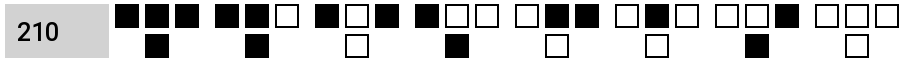
\includegraphics[width=\textwidth]{img/eca1.png}
		\caption{ECA 210}
		\label{img:eca1}
	\end{figure}
	
	\begin{figure}[H]
		\centering
		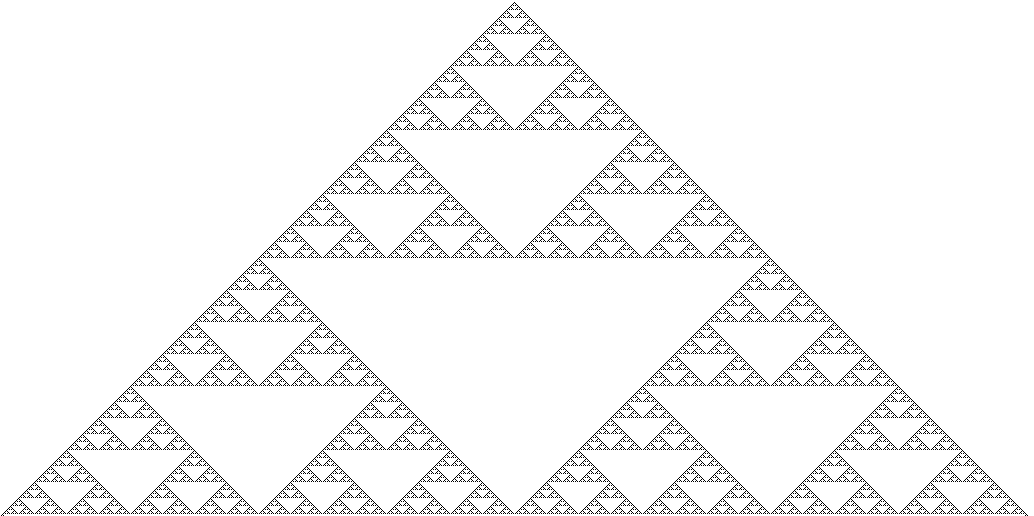
\includegraphics[width=\textwidth]{img/eca2.png}
		\caption{Evolución del ECA 210}
		\label{img:eca2}
	\end{figure}
	
	\subsection{Regla 30}
	
	La regla 30 equivale a $30_{10}=00011110_2$ en binario. Dada una única célula con valor 1, esta se expande en ambas direcciones con cada iteración, como se muestra en las figuras \ref{img:r30_1} y \ref{img:r30_2}, que ilustran las primeras 23 y 900 generaciones, respectivamente.
	
	Como se observa en la figura \ref{img:r30_2}, existe un pequeño patrón repetitivo que crece de forma diagonal en el lado izquierdo del historial. Sin embargo, en el lado derecho, el comportamiento no parece tener estabilidad ni un patrón discernible. Si almacenamos el historial de los valores de la célula inicial, se obtiene una secuencia pseudoaleatoria.
	
	Hasta el momento no se ha podido predecir directamente si el siguiente estado será 0 o 1, es posible calcularlo realizando todas las generaciones previas.
	
	\begin{figure}[H]
		\centering
		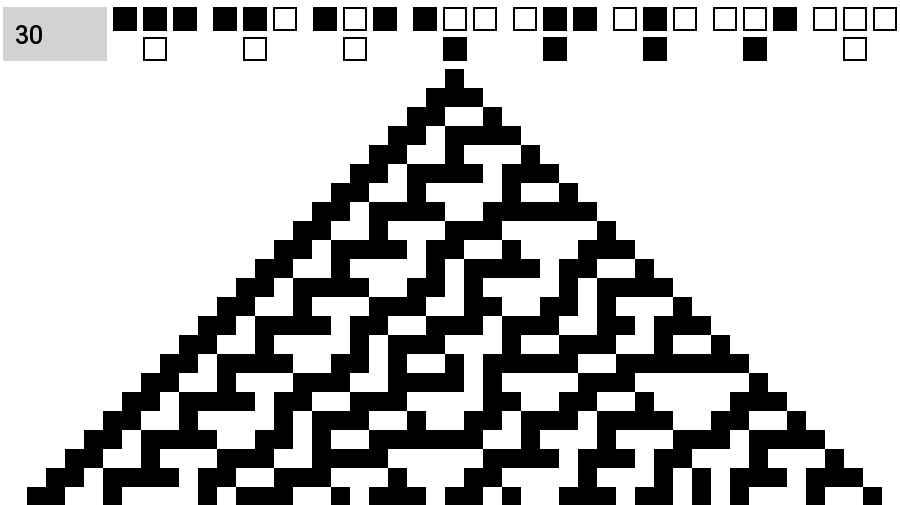
\includegraphics[width=\textwidth]{img/r30_1.png}
		\caption{Primeras 23 generaciones de la regla 30}
		\label{img:r30_1}
	\end{figure}
	
	\begin{figure}[H]
		\centering
		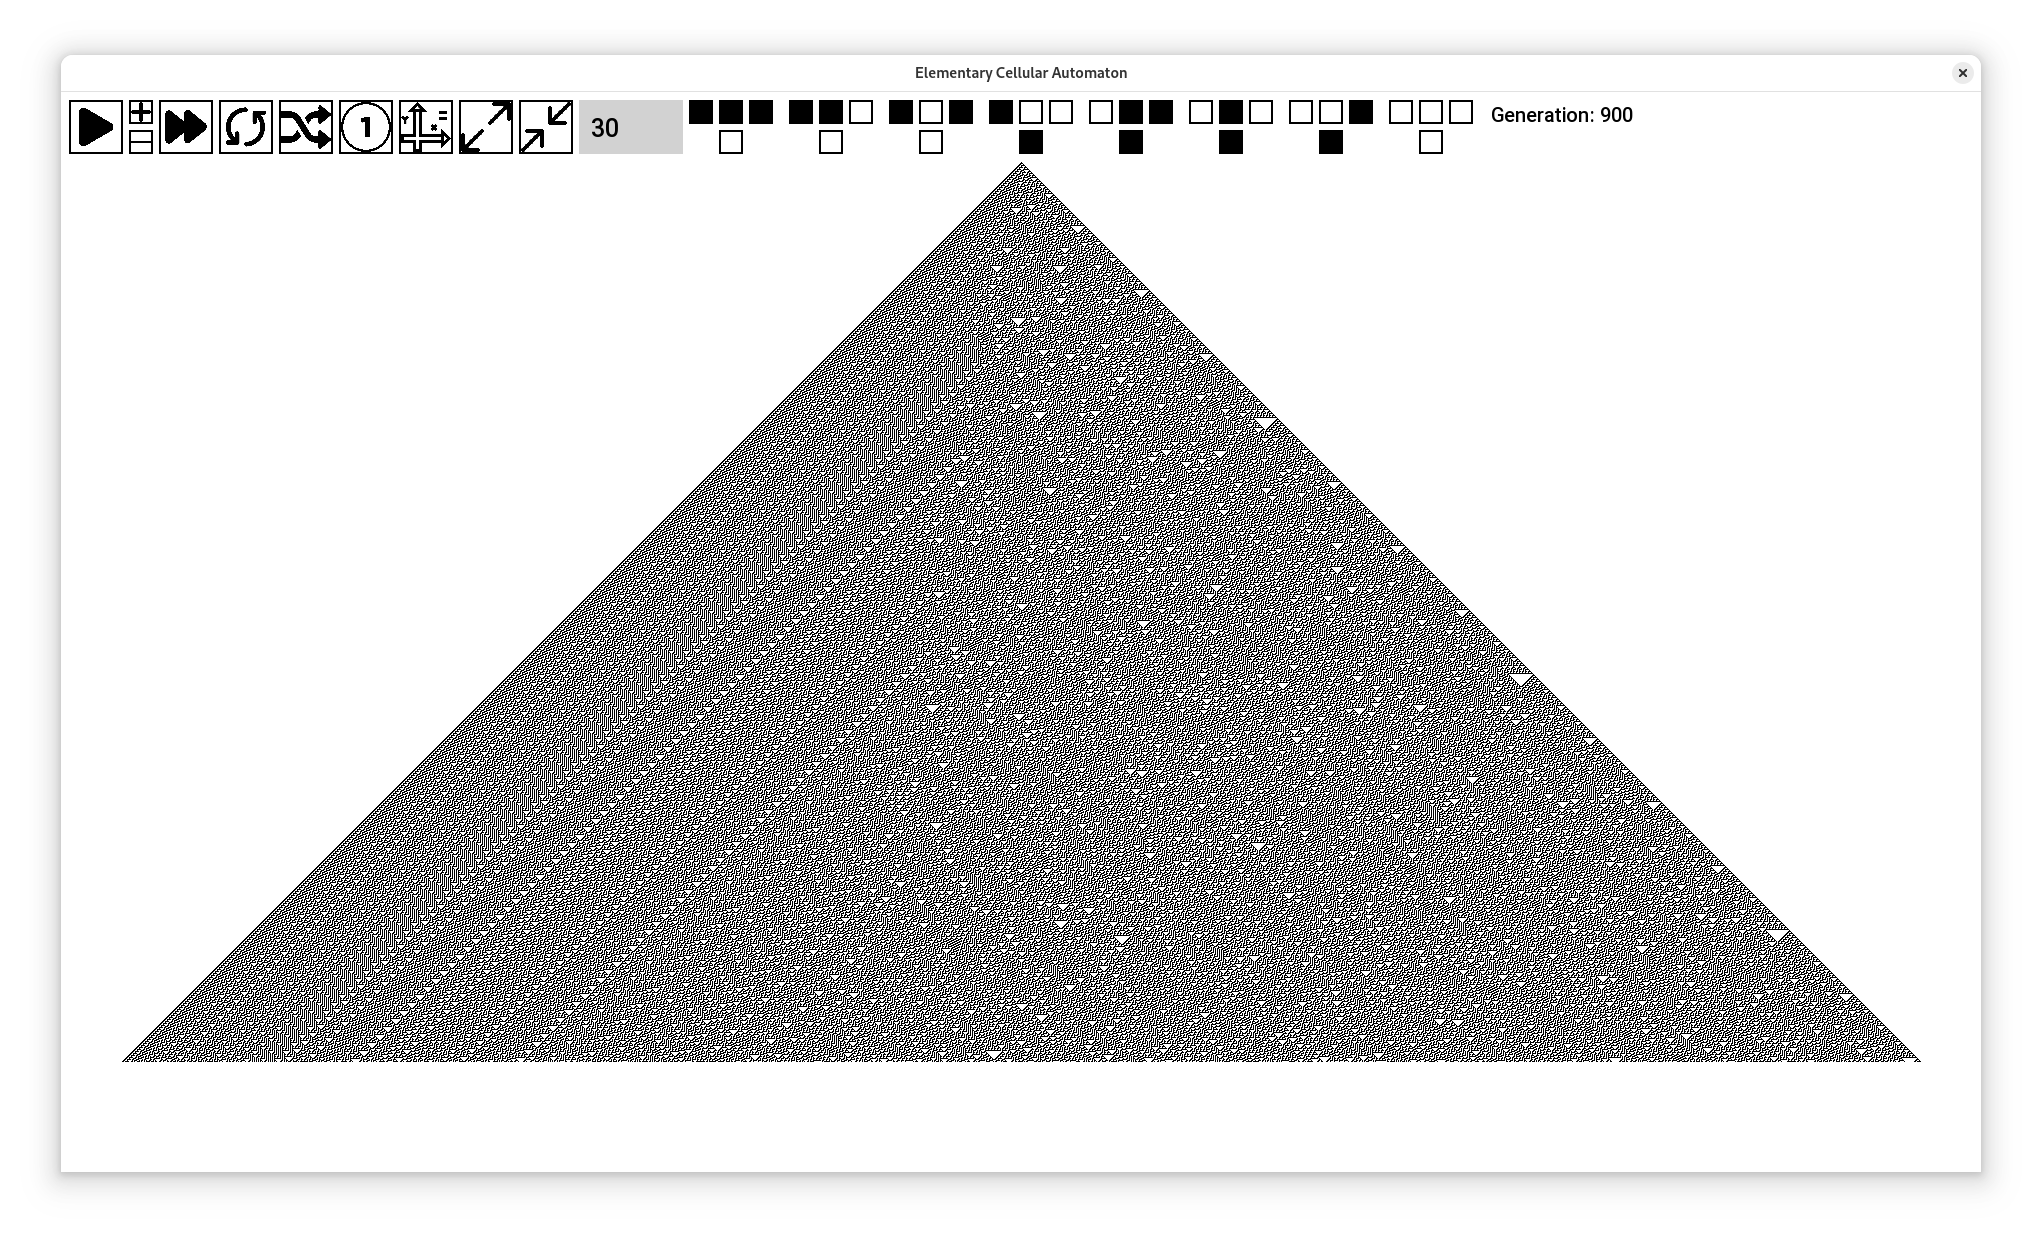
\includegraphics[width=\textwidth]{img/r30_2.png}
		\caption{Primeras 900 generaciones de la regla 30}
		\label{img:r30_2}
	\end{figure}
	
	\section{Metodología}
	
	\subsection{Extracción de la columna principal}
	
	Mediante la función \ref{fun:ca}, se generan las primeras $t$ generaciones de la regla 30 del ECA y extrae, en formato de lista, el historial de la columna principal. Para las pruebas se extrajo un vector de $t=5$ millones de generaciones.
	
\begin{lstlisting}[style=modernMathematica, label=fun:ca, caption={Función extractora de la columna principal}]
column=CellularAutomaton[30, {{1}, 0}, {t, {{0}}}]
\end{lstlisting}

\subsection{Generación de divisores}

Se define un conjunto de divisores con la función \ref{fun:div}. Este se compone de los primeros 100 números naturales, junto con todos los números primos menores que la raíz cuadrada del total de generaciones. Es decir, todos los primos menores que $\sqrt{5,000,000} = 2221$, lo que da un total de 406 divisores.  

Los números primos fueron elegidos por dos razones. La primera es que se busca reducir la complejidad computacional. La segunda se basa en el teorema fundamental de la aritmética, que establece que todo número puede expresarse como el producto de números primos. Esto implica que, si existe algún patrón en un número, dicho patrón también debería existir en sus componentes primarias.  

Finalmente, el límite de $2221$ se define porque, para ese número, existe la misma cantidad de particiones que pueden realizarse en la columna principal. Cuanto mayor sea el divisor, menor será el número de particiones, lo que a su vez implica menos datos para el análisis.

\begin{lstlisting}[style=modernMathematica, label=fun:div, caption={Selección de divisores}]
divisors=Join[
  Range[1, 100],
  Prime @ Range @ PrimePi[Sqrt[Length[column]]]
] // Sort
\end{lstlisting}
	
\subsection{Histogramas}

	Para generar los histogramas, se siguen los siguientes pasos:
	\begin{enumerate}
		\item Se selecciona un $divisor$.
		\item Se particiona el vector de la columna principal en segmentos de tamaño $divisor$.
		\item Se cuenta el número de unos en cada partición (Función \ref{fun:density}).
		\item Se registran las frecuencias de todos los conteos realizados (Función \ref{fun:frecuencies}).
	\end{enumerate}
	
\begin{lstlisting}[style=modernMathematica, label=fun:density, caption={Partición y conteo}]
Density = Function[{column, divisor},
  partitions = Partition[column, divisor];
  density = Table[
    Count[partitions[[i]], 1], 
    {i, 1, Length[partitions]}
  ]
];
\end{lstlisting}

\begin{lstlisting}[style=modernMathematica, label=fun:frecuencies, caption={Selección de divisores}]
Frecuencies = Function[{column},
  unique = DeleteDuplicates[column];
  frecuencies = Table[
    {unique[[i]], Count[column, unique[[i]]]}, 
    {i, 1, Length[unique]}
  ]
];
\end{lstlisting}


	Al graficar los puntos, se puede intuir una distribución normal de las frecuencias, como se muestra en la figura \ref{img:test1_10}. En este caso, se utiliza un vector de la columna principal con 100,000 elementos, particionado en 10. Por otro lado, en la figura \ref{img:test1_500}, utilizando un vector del mismo tamaño pero particionado en 500, se observa un comportamiento caótico.  
	
	Esta diferencia podría deberse a la cantidad de datos con los que trabaja cada partición. Con particiones de tamaño 10, se obtienen $\frac{100,000}{10} = 10,000$ subvectores. En cambio, con particiones de tamaño 500, se obtienen $\frac{100,000}{500} = 200$ subvectores, 50 veces menos que en el primer caso.  
	
	Para realizar una comparación adecuada, lo ideal sería trabajar con más datos a medida que aumenta el tamaño de la partición, de modo que todas generen el mismo número de subvectores. Sin embargo, aumentar el número de generaciones incrementa el tiempo de procesamiento. Para evitar esto, en lugar de aumentar el tamaño del vector de la columna principal, se opta por dividirlo en un vector más pequeño y repetir los pasos mencionados, pero con diferentes tamaños del vector principal.  
	
	Este nuevo enfoque permite analizar el comportamiento del histograma a medida que se incrementa el tamaño del vector.

	\begin{figure}[H]
		\centering
		\begin{minipage}{0.45\textwidth}
			\centering
			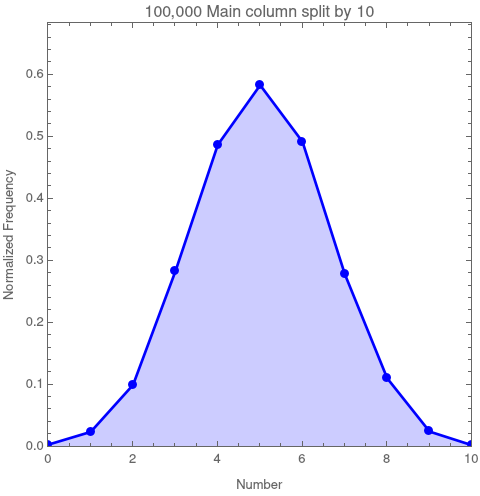
\includegraphics[width=\textwidth]{img/test_1_10.png}
			\caption{Histograma: 100,000 generaciones particionadas en 10}
			\label{img:test1_10}
		\end{minipage}
		\hfill
		\begin{minipage}{0.45\textwidth}
			\centering
			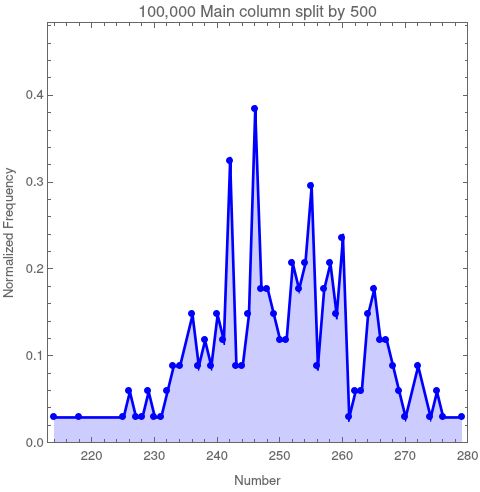
\includegraphics[width=\textwidth]{img/test_1_500.png}
			\caption{Histograma: 100,000 generaciones particionadas en 500}
			\label{img:test1_500}
		\end{minipage}
	\end{figure}

	\subsection{Histograma evolutivo}
	
	Al implementar los histogramas evolutivos, se añadieron dos parámetros adicionales: el tamaño mínimo del vector y el incremento. Estos valores sirven para reducir el número de operaciones realizadas, ya que resulta poco práctico y poco útil aumentar el tamaño del vector de divisor en divisor. Además, no se extrae suficiente información al obtener solo un dato más. Estos valores son generados y normalizados mediante la función \ref{fun:his_frec}.  
	
	Para las 5 millones de generaciones, se optó por un valor inicial de 1 millón y un incremento de 10,000. Esto nos permite obtener  
	\[
	\frac{(5,000,000 - 1,000,000)}{10,000} + 1 = 401
	\]  
	muestras a lo largo del tiempo.  
	
	Para el divisor más grande ($2221$), la muestra inicial contiene  $\frac{1,000,000}{2,221} = 450$ datos, mientras que cada muestra de tiempo adicional contiene  $\frac{10,000}{2,221} = 4$ datos (solo se toma la parte entera), dando un total de 2251 datos.  
	
	Finalmente, se utiliza la función \ref{fun:all_his_frec}, que calcula los histogramas evolutivos para todos los divisores generados. Se ajusta el tamaño de cada incremento para que sea un múltiplo entero del divisor.  
	
\begin{lstlisting}[style=modernMathematica, label=fun:his_frec, caption={Calculo y normalización de frecuencias evolutivas}]
HistoricFrecuency = Function[
  {column, divisor, min, increment},
  historic = Table[
  Frecuencies @ Density[column[[1 ;; i]], divisor], 
  {i, min,Length[column], increment}];
  
  Do[
    historic[[i, All, 2]] = Normalize[historic[[i, All, 2]]];,
    {i, 1, Length[historic]}];
  historic
];
\end{lstlisting}


\begin{lstlisting}[style=modernMathematica, label=fun:all_his_frec, caption={Todos los histogramas evolutivos}]
AllHistoric = Function[
  {column, divisors, min, increment},
  Table[{
  	  divisors[[i]],
	  min - Mod[increment, divisors[[i]]],
	  increment - Mod[increment, divisors[[i]]],
	  HistoricFrecuency[
	    column, 
	    divisors[[i]], 
 	    min - Mod[increment, divisors[[i]]], 
	    increment - Mod[increment, divisors[[i]]]]
	}, {i, 1, Length[divisors], 1}]
];
\end{lstlisting}

	\subsection{Métricas}
	Por ultimo, se calculan ciertas métricas para todos los divisores y todas las muestras de cada divisor mediante la función \ref{fun:statistic}. Estos datos son: media, varianza, desviación estándar, asimetría y kurtosis. 

\begin{lstlisting}[style=modernMathematica, label=fun:statistic, caption={Calculos estadisticos}]
calculateStatistics[data_] := Module[{wd},
  wd = WeightedData[data[[All, 1]], data[[All, 2]]];
 
  <|"mean" -> Mean[wd],
  "variance" -> Variance[wd],
  "standardDeviation" -> StandardDeviation[wd],
  "skewness" -> Skewness[wd],
  "kurtosis" -> Kurtosis[wd]|>
];
\end{lstlisting}

	\clearpage
	\addcontentsline{toc}{section}{Referencias}
	\begin{thebibliography}{99}
		\bibitem{b1}
		M. G. Magaña Chávez. ``Autómatas celulares elementales y sus composiciones''. Motivos matemáticos / Matemáticas aplicadas. Accedido el 24 de diciembre de 2024. [En línea]. Disponible: \url{https://motivos.matem.unam.mx/vol6/num1/aplicadas1.html#:~:text=En%201948,%20el%20célebre%20matemático,de%20construir%20a%20otro%20robot}
		
		\bibitem{b2}
		C. A. Rodríguez Garzón, ``Modelamiento de estaciones TransMilenio mediante Autómatas Celulares: lecciones aprendidas'', Ingeniería, vol. 19, n.º 2, diciembre de 2014. Accedido el 28 de diciembre de 2024. [En línea]. Disponible: \url{https://doi.org/10.14483/udistrital.jour.reving.2014.2.a05}
		
		\bibitem{b3}
		V. E. Barros Arenas y H. Gilabert P., ``Modelación de la dinámica Plaga-Parasitoide-Bosque mediante autómatas celulares'', Cienc. \& Investig. For., vol. 14, n.º 2, pp. 311–323, julio de 2008. Accedido el 28 de diciembre de 2024. [En línea]. Disponible: \url{https://doi.org/10.52904/0718-4646.2008.292}
		
		\bibitem{b4}
		J. J. M. Martínez, ``Modelo de autómatas celulares para la dinámica de un mercado financiero'', Económica, pp. 46–94, diciembre de 2018. Accedido el 28 de diciembre de 2024. [En línea]. Disponible: \url{https://doi.org/10.24215/18521649e004}
		
		\bibitem{b5}
		T. Muñoz Jiménez, A. Torres Soto y M. D. Torres Soto, ``Autómatas Celulares Aplicados al Comportamiento de Células de Cáncer Cervicouterino'', Tecnol. Educ. Rev. CONAIC, vol. 6, n.º 1, pp. 44–49, enero de 2021. Accedido el 28 de diciembre de 2024. [En línea]. Disponible: \url{https://doi.org/10.32671/terc.v6i1.48}
		
		\bibitem{b6}
		``Conway's Game of Life - LifeWiki''. Conway's Game of Life. Accedido el 25 de diciembre de 2024. [En línea]. Disponible: \url{https://conwaylife.com/wiki/Conway's_Game_of_Life}
		
		\bibitem{b7}
		Wolfram Research, Inc. ``Elementary Cellular Automaton''. Wolfram MathWorld. Accedido el 28 de diciembre de 2024. [En línea]. Disponible: \url{https://mathworld.wolfram.com/ElementaryCellularAutomaton.html}
		
		\bibitem{b8}
		Wolfram Research, Inc. ``Rule 30''. Wolfram MathWorld. Accedido el 28 de diciembre de 2024. [En línea]. Disponible: \url{https://mathworld.wolfram.com/Rule30.html}
		
	\end{thebibliography}
	
\end{document}
